\documentclass[a4,12pt]{horizon-theme}
\usepackage{lipsum}
\usepackage{fontawesome5}
\usepackage{graphicx,url}
\usepackage{float}
\usepackage{amsmath}
\usepackage{booktabs}
\usepackage{makecell}
\usepackage{array}
\usepackage{multirow}
\usepackage{caption}
\usepackage{subcaption}
\usepackage{siunitx}
\usepackage{enumerate}
\usepackage{gensymb}
\usepackage{csvsimple}
\usepackage{tabularray}
\usepackage{stackengine}
\usepackage{xcolor, colortbl}
\usepackage[round]{natbib}
\usepackage{karnaugh-map}
\usepackage{stackengine}
% \usepackage{longtable}
\usepackage{minted}

\strutlongstacks{T}

\BeforeBeginEnvironment{minted}{\vspace{-20pt}}


% Cover Config
% \configCover{<num. do exp.>}{<data>}{<título>}
\configCover{6}{02/06/2022}{Projeto de Máquinas de Estados em VHDL}



\begin{filecontents*}{tb_testes.csv}
clock,zera,vagas,conta-vagas,direcao-vagas,conta-idoso,direcao-idoso,contagem-vagas,contagem-idoso,cheio
$\times$,1,$\times$,$\times$,$\times$,$\times$,$\times$,000,000,0
$\uparrow$,0,110,1,1,0,0,001,000,0
$\uparrow$,0,110,1,1,0,0,010,000,0
$\uparrow$,0,110,1,1,0,0,011,000,0
$\uparrow$,0,110,0,0,1,1,100,001,0
$\uparrow$,0,110,0,0,1,1,101,010,0
$\uparrow$,0,110,1,1,0,0,110,010,1
$\uparrow$,0,110,1,0,0,0,110,010,1
$\uparrow$,0,110,1,0,0,0,101,000,0
$\uparrow$,0,110,1,0,0,0,100,000,0
$\uparrow$,0,110,1,0,0,0,011,000,0
$\uparrow$,0,110,1,0,0,0,010,000,0
$\uparrow$,0,110,0,0,1,0,001,001,0
$\uparrow$,0,110,0,0,1,0,000,000,0
\end{filecontents*}



\newenvironment{code}{\captionsetup{type=listing}}{}


\begin{document}
\horizonCover

\horizonTitle


\section{Introdução} % R
O VHDL é uma linguagem de descrição de hardware. Com ela é possível descrever e simular circuitos digitais dos mais diversos sem a necessidade de se montar o circuito e testá-lo a cada alteração na descrição. Nesse experimento, será realizado um projeto simples utilizadno o VHDL.

\section{Objetivos} % N
O objetivo deste experimento é modificar o projeto anterior de controle de vagas de estacionamento adicionando contagem de veículos pertencentes a idosos e implementá-lo usando a divisão em fluxo de dados e unidade de controle.


\section{Planejamento} % N, R
\label{sec:plan}

\subsection{Fluxo de dados}
\label{sec:fd}


\subsubsection{Diagrama de blocos}
\label{sec:fd_blocos}

\begin{figure}[!ht]
    \centering
    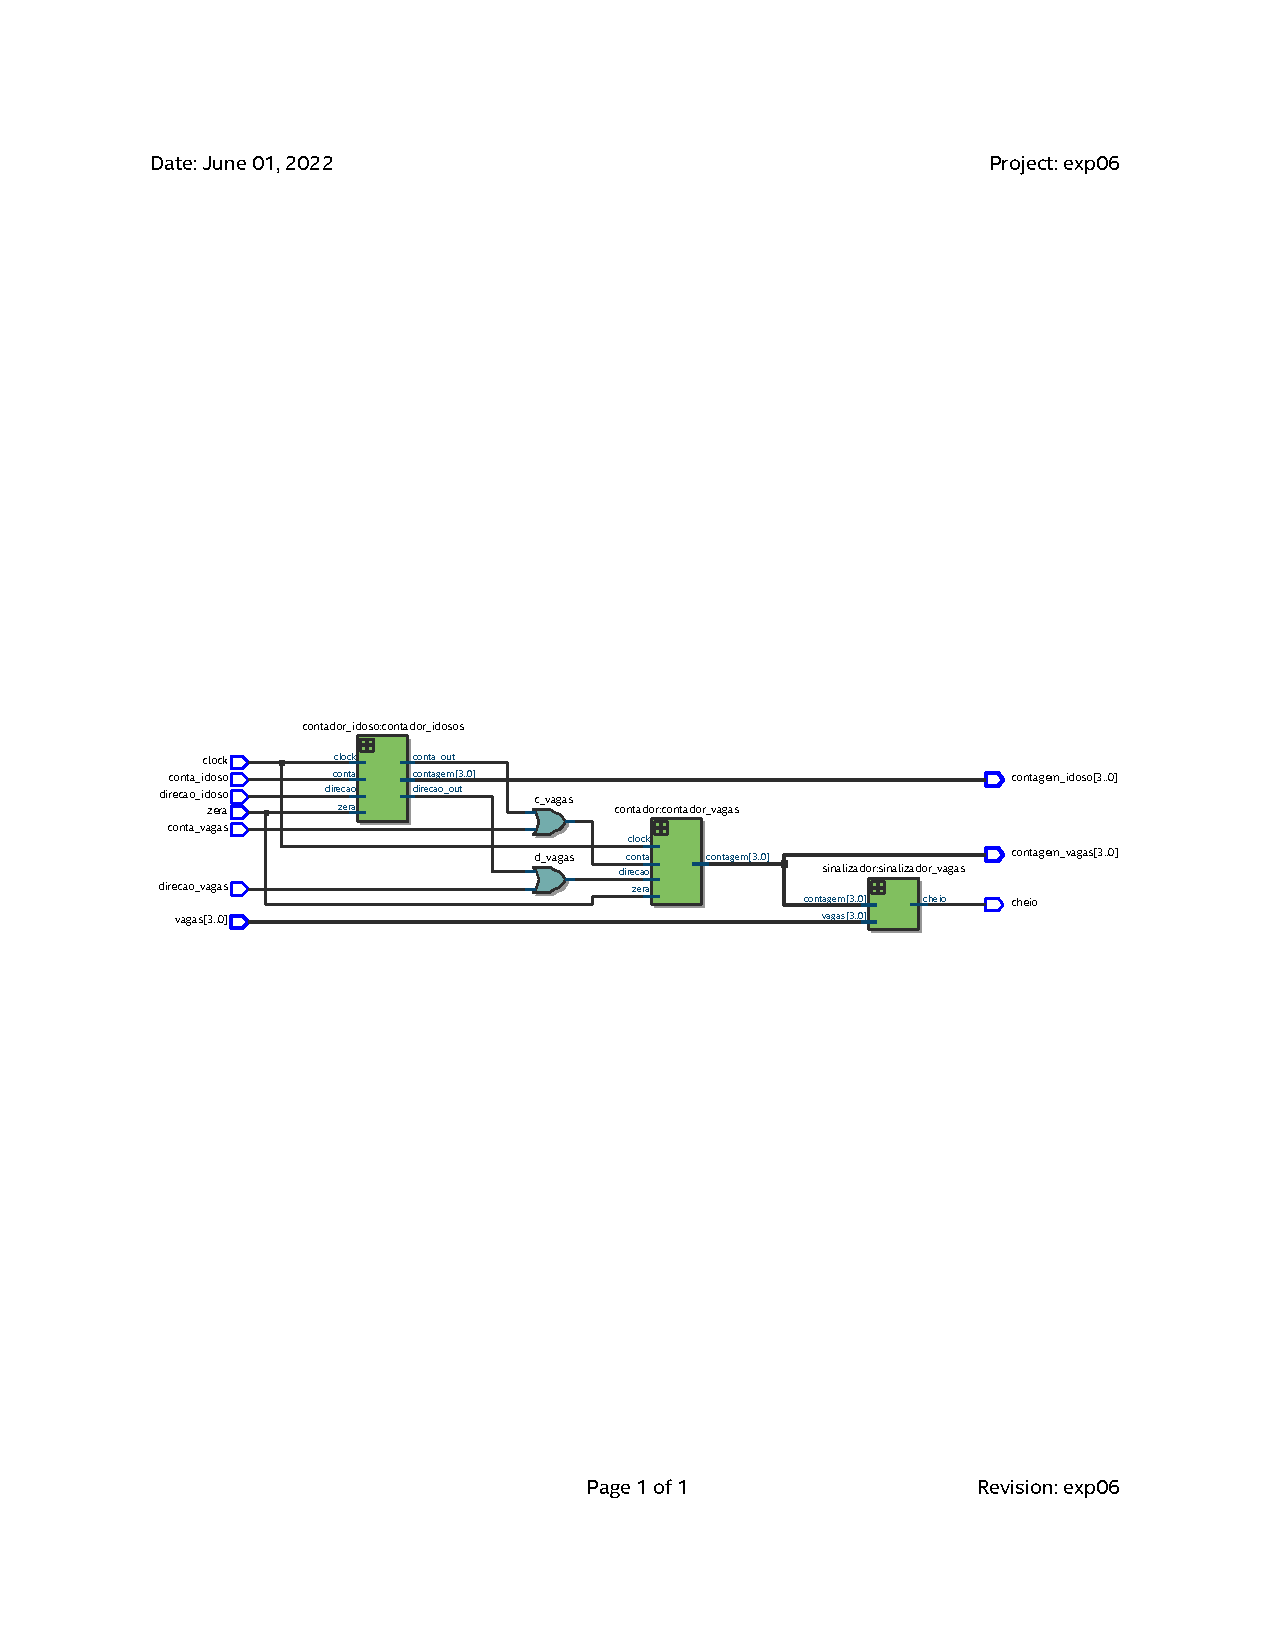
\includegraphics[width=\textwidth, trim={25mm, 120mm, 25mm, 120mm}, clip]{fd_blocos}
    \caption{Diagrama de blocos do Fluxo de Dados}
    \label{fig:fd_blocos}
\end{figure}

A Fig. \ref{fig:fd_blocos} mostra o Diagrama de Blocos gerado a partir da descrição em VHDL do fluxos de dados (\ref{lst:fd}).


\subsubsection{Carta dos Tempos}
\label{sec:fd_tempos}

A partir da simulação, foi possível gerar a carta de tempos para o componente fluxo de dados, que é mostrada na Fig. \ref{fig:fd_tempos}. Nela é testada se o contador dá prioridade ao contador idoso. Também é notado que o contador não para no limite de vagas, pois este comportamento é controlado pela unidade de controle.

\begin{figure}[!ht]
    \centering
    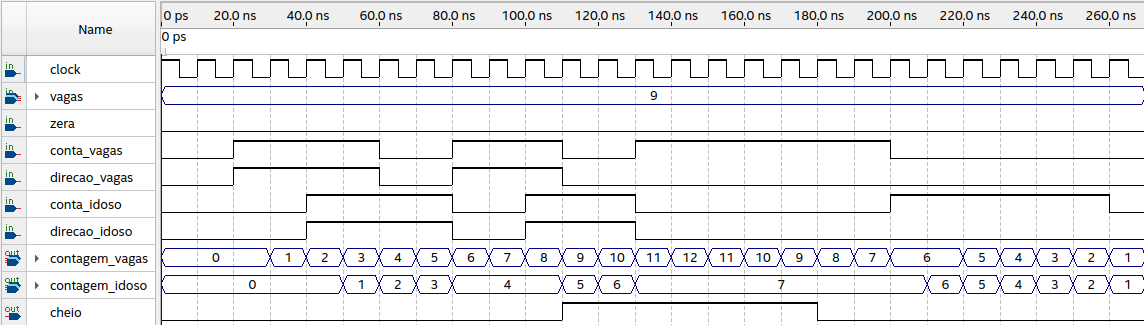
\includegraphics[width=\textwidth]{fd}
    \caption{Carta de tempos do Fluxo de Dados}
    \label{fig:fd_tempos}
\end{figure}




\subsection{Unidade de Controle}
\label{sec:uc}

\subsubsection{Diagrama de blocos}
\label{sec:uc_blocos}

A Fig. \ref{fig:uc_blocos} mostra o Diagrama de Blocos gerado a partir da descrição em VHDL do fluxos de dados (\ref{lst:uc}).

\begin{figure}[!ht]
    \centering
    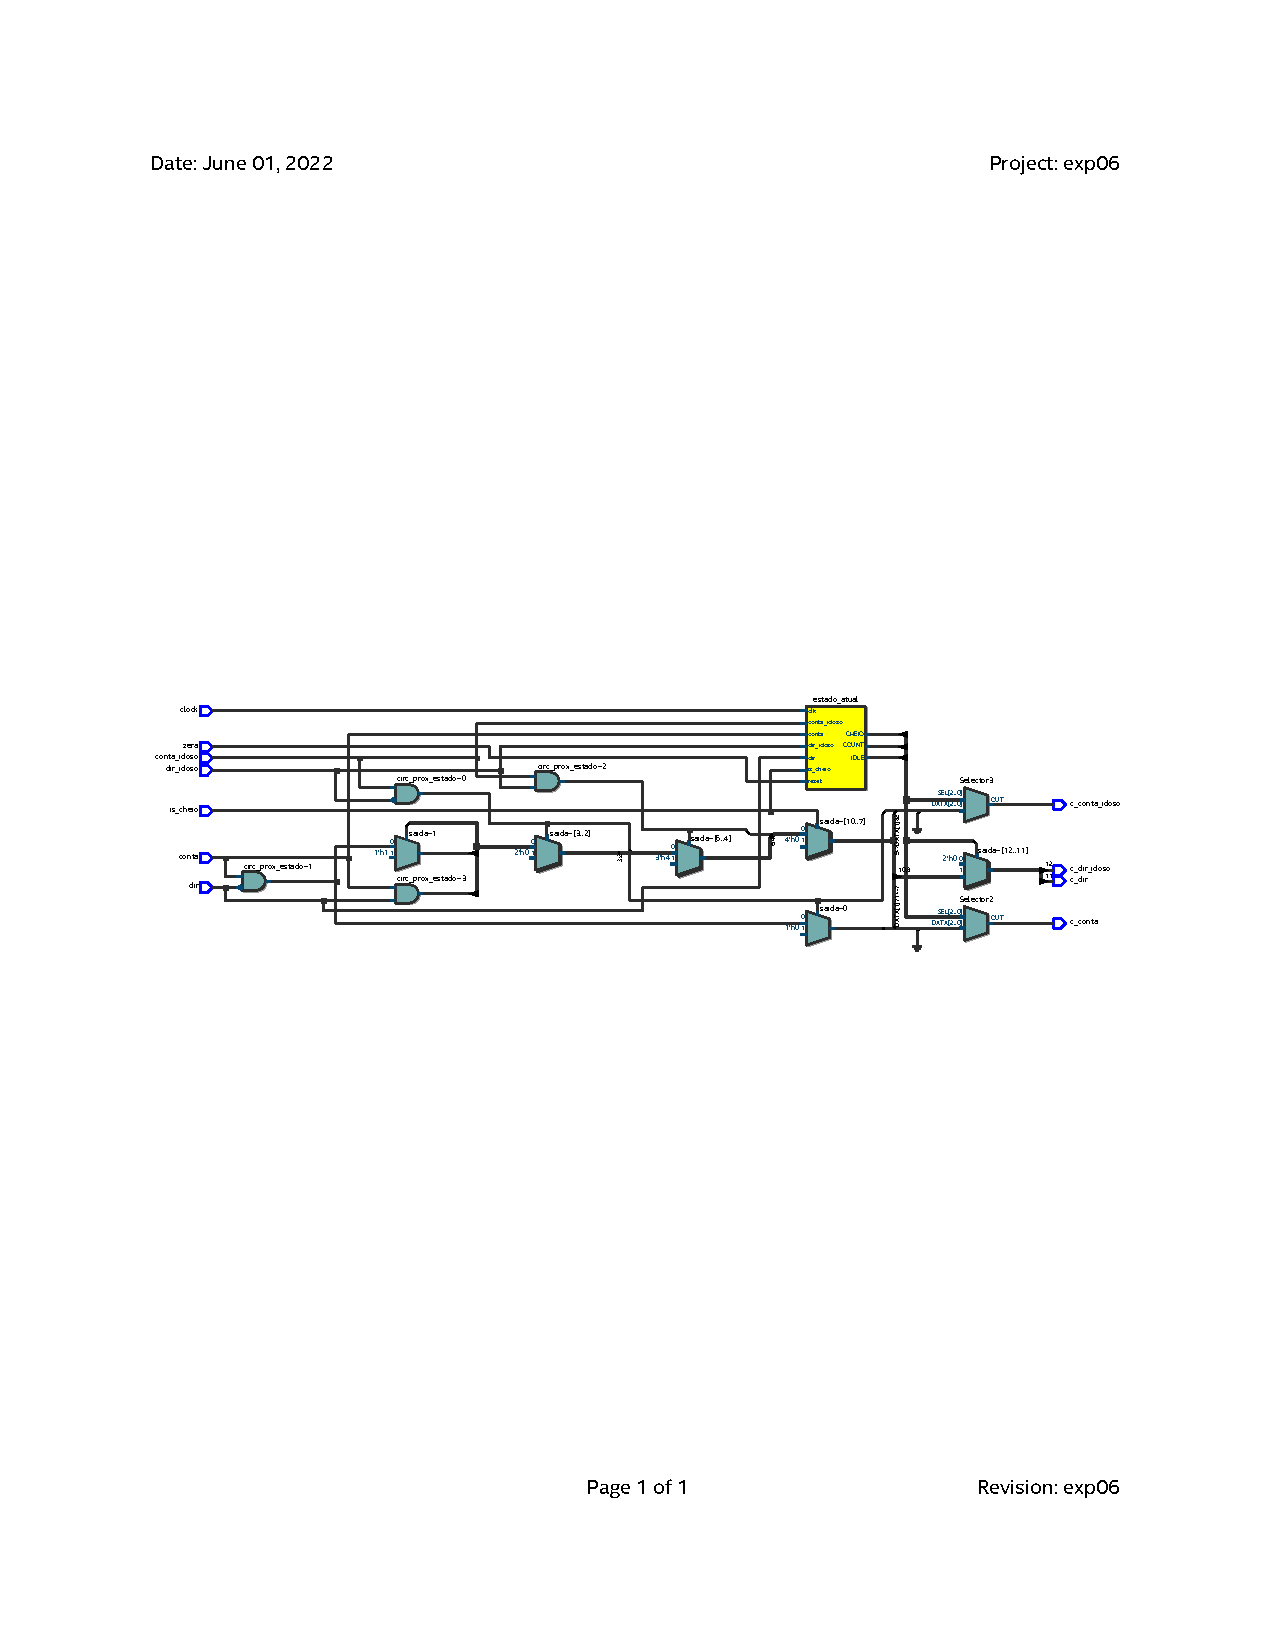
\includegraphics[width=\textwidth, trim={25mm, 105mm, 25mm, 105mm}, clip]{uc_blocos}
    \caption{Diagrama de blocos da Unidade de Controle}
    \label{fig:uc_blocos}
\end{figure}




\subsubsection{Diagrama de estados}
\label{sec:uc_estados}

A Fig. \ref{fig:uc_estados} mostra o diagrama de estados para a Máquina de Estados implementada na Unidade de Controle. Ela possui dois estados: ``CHEIO'' e ``COUNT'', sendo que o terceiro estado foi colocado apenas por restrições da ferramenta Quartus.

\begin{figure}[!ht]
    \centering
    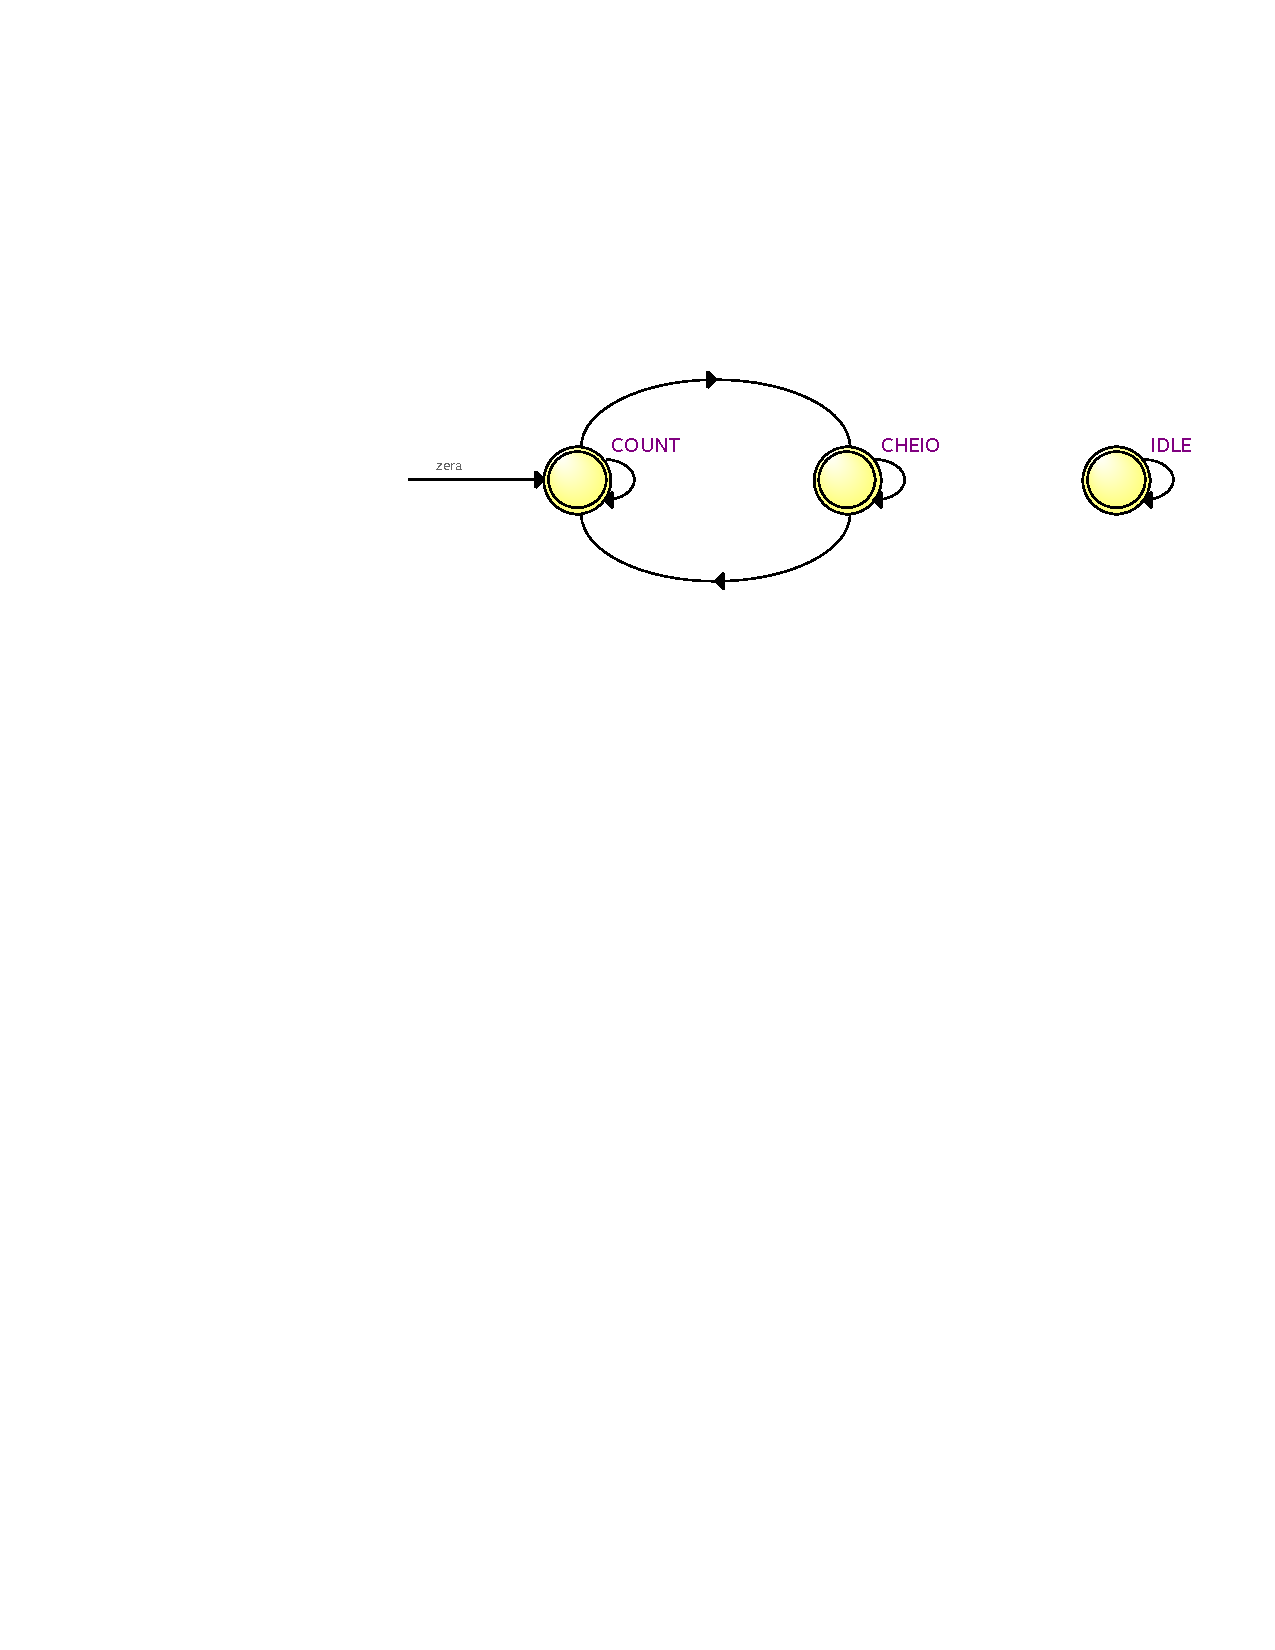
\includegraphics[width=\textwidth, trim={65mm, 176mm, 5mm, 60mm}, clip]{uc_estados}
    \caption{Diagrama de estados da Unidade de Controle}
    \label{fig:uc_estados}
\end{figure}





\subsubsection{Carta dos Tempos}
\label{sec:uc_tempos}

A partir da simulação, foi possível gerar a carta de tempos para o componente unidade de controle, que é mostrada na Fig. \ref{fig:uc_tempos}. Nela são testados os sinais de controle gerados a partir dos estímulos externos para controlar o componente fluxo de dados.

\begin{figure}[!ht]
    \centering
    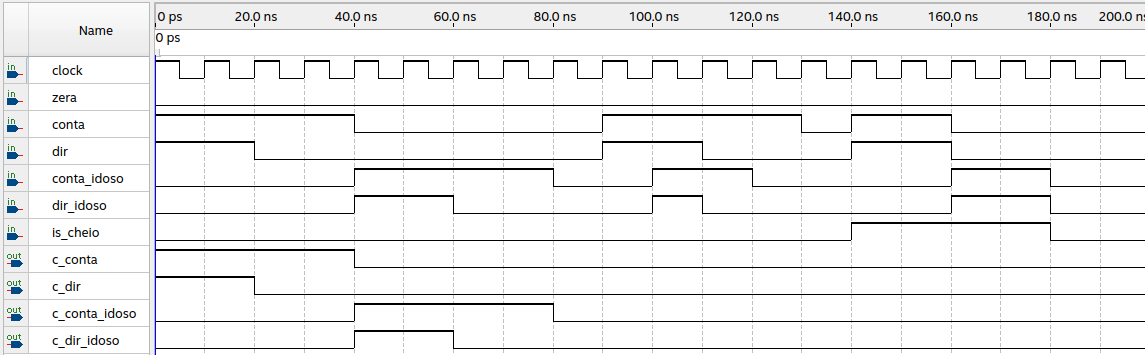
\includegraphics[width=\textwidth]{uc}
    \caption{Carta de tempos da Unidade de Controle}
    \label{fig:uc_tempos}
\end{figure}



\newpage
\section{Resultados}
\label{sec:resultados}

Foi implementada descrição em VHDL do circuito completo, que inclui os componentes \emph{Fluxo de Dados} e \emph{Unidade de Controle}. A Fig. \ref{fig:completo} mostra a carta de tempos deste circuito completo.

\begin{figure}[!ht]
    \centering
    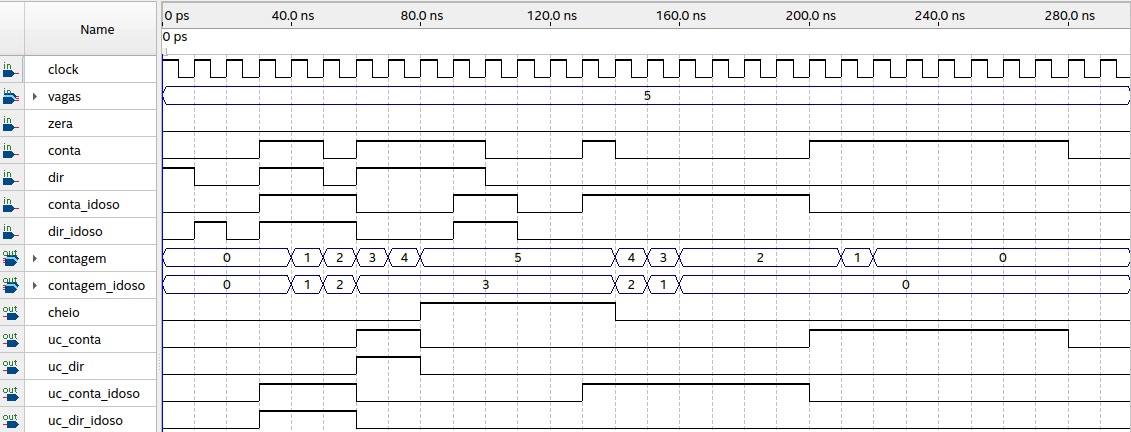
\includegraphics[width=\textwidth]{completo}
    \caption{Carta de tempos do circuito completo}
    \label{fig:completo}
\end{figure}

Após a implementação da descrição, o circuito foi implantado em uma placa FPGA. A Tabela \ref{tab:testes} mostra os valores esperados para cada teste. Todas as respostas do circuito implantado foram condizentes com a tabela de testes.

\begin{table}[!ht]
    \centering
    \caption{Tabela de testes do circuito completo}
    \label{tab:testes}
    \doubleRuleSep
    \begin{tabular}{*{10}{c}}
        \doubleTopRule
        \multicolumn{7}{c}{Entradas} & \multicolumn{3}{c}{Saídas}\\
        \cmidrule(lr){1-7}\cmidrule(lr){8-10}
        clk & zera & vagas & conta & direcao & conta (i) & direcao (i) & contagem & contagem (i) & cheio\\
        \midrule
        \csvreader[head to column names, late after line=\\]{tb_testes.csv}{}%
        {\csvcoli & \csvcolii & \csvcoliii & \csvcoliv & \csvcolv & \csvcolvi & \csvcolvii & \csvcolviii & \csvcolix & \csvcolx}%
        \doubleBottomRule
    \end{tabular}
\end{table}


\section{Conclusão}
Um circuito digital para controle de vagas de estacionamento com contagem separada de idosos foi implementado em VHDL e implantado em uma placa FPGA com todas as saídas desse circuito coerentes com os resultados de simulação.


\newpage
\appendix
\section*{Apêndice}
\renewcommand{\thesubsection}{\Alph{subsection}}

\subsection{Descrições dos circuitos}
\label{ap:vhdl}

Descrições comentadas dos circuitos comparador e contador em VHDL

\begin{code}
\captionof{listing}{Descrição do Fluxo de Dados}
\label{lst:fd}
\begin{minted}[frame=lines, framesep=6pt, framerule=0.5pt, linenos, rulecolor=secondaryColor, breaklines]{VHDL}
library IEEE;
use IEEE.std_logic_1164.all;
use IEEE.numeric_std.all;

entity fluxo_dados is
  port(
    clock, zera: in std_logic;
    vagas: in std_logic_vector(3 downto 0);
    conta_vagas, direcao_vagas: in std_logic;
    conta_idoso, direcao_idoso: in std_logic;
    contagem_vagas, contagem_idoso: out std_logic_vector(3 downto 0);
    cheio: out std_logic
  );
end fluxo_dados;

architecture fluxo_dados_arch of fluxo_dados is
  component contador is
    port(
      clock, zera, conta, direcao: in std_logic;
      contagem: out std_logic_vector(3 downto 0)
    );
  end component;

  component contador_idoso is
    port(
      clock, zera, conta, direcao: in std_logic;
      contagem: out std_logic_vector(3 downto 0);
      conta_out, direcao_out: out std_logic
    );
  end component;

  component sinalizador is
    port(
      vagas, contagem: in std_logic_vector(3 downto 0);
      cheio: out std_logic
    );
  end component;

  signal qtd_vagas, qtd_idoso: std_logic_vector(3 downto 0);
  signal c_idoso, d_idoso, c_vagas, d_vagas: std_logic;
begin
  contagem_vagas <= qtd_vagas;
  contagem_idoso <= qtd_idoso;
  c_vagas <= conta_vagas or c_idoso;
  d_vagas <= direcao_vagas or d_idoso;
  
  contador_vagas: contador port map(
    clock => clock, 
    zera => zera, 
    conta => c_vagas, 
    direcao => d_vagas, 
    contagem => qtd_vagas
  );

  contador_idosos: contador_idoso port map(
    clock => clock, 
    zera => zera, 
    conta => conta_idoso,
    direcao => direcao_idoso, 
    contagem => qtd_idoso,
    conta_out => c_idoso,
    direcao_out => d_idoso
  );

  sinalizador_vagas: sinalizador port map(
    vagas => vagas,
    contagem => qtd_vagas,
    cheio => cheio
  );
end fluxo_dados_arch;
\end{minted}
\end{code}


\newpage
\begin{code}
\captionof{listing}{Descrição da Unidade de Controle}
\label{lst:uc}
\begin{minted}[frame=lines, framesep=6pt, framerule=0.5pt, linenos, rulecolor=secondaryColor, breaklines]{VHDL}
library IEEE;
use IEEE.std_logic_1164.all;
use IEEE.numeric_std.all;

entity unidade_controle is
  port(
    clock, zera, is_cheio: in std_logic;
    conta, dir, conta_idoso, dir_idoso: in std_logic;
    c_conta, c_dir, c_conta_idoso, c_dir_idoso: out std_logic
  );
end unidade_controle;


architecture unidade_controle_arch of unidade_controle is
  type estado_t is (COUNT, CHEIO, IDLE);
  signal estado_prox, estado_atual: estado_t;
  signal saida: std_logic_vector(3 downto 0);
begin
  sincrono: process(clock, zera, estado_prox)
  begin
    if zera='1' then
      estado_atual <= COUNT;
    elsif clock'event and clock='1' then
      estado_atual <= estado_prox;
    end if;
  end process;

  circ_prox_estado: process(estado_atual, conta, dir, conta_idoso, dir_idoso, is_cheio)
  begin
    case estado_atual is
      when CHEIO =>
        if conta_idoso='1' and dir_idoso='0' then
          estado_prox <= COUNT;
          saida <= "0010";
        elsif conta='1' and dir='0' then
          estado_prox <= COUNT;
          saida <= "1000";
        else
          estado_prox <= CHEIO;
          saida <= "0000";
        end if;
      when COUNT =>
        if is_cheio='1' then
          estado_prox <= CHEIO;
          saida <= "0000";
        elsif conta_idoso='1' and dir_idoso='1' then
          estado_prox <= COUNT;
          saida <= "0011";
        elsif conta_idoso='1' and dir_idoso='0' then
          estado_prox <= COUNT;
          saida <= "0010";
        elsif conta='1' and dir='1' then
          estado_prox <= COUNT;
          saida <= "1100";
        elsif conta='1' and dir='0' then
          estado_prox <= COUNT;
          saida <= "1000";
        else
          estado_prox <= COUNT;
          saida <= "0000";
        end if;
      when IDLE =>
        estado_prox <= IDLE;
        saida <= "0000";
      end case;
  end process;

  c_conta <= saida(3);
  c_dir <= saida(2);
  c_conta_idoso <= saida(1);
  c_dir_idoso <= saida(0);
end unidade_controle_arch;
\end{minted}
\end{code}


% \bibliographystyle{plainnat}
% \bibliography{refs}

\horizonBackCover
\end{document}